\documentclass[a4paper,11pt, twoside]{article}
\newcommand{\n}[1]{\textbf{#1}}
\usepackage{graphicx}
\usepackage{amsfonts}
\usepackage{amsmath}
\usepackage[brazilian]{babel}
\usepackage[utf8]{inputenc}
\usepackage[T1]{fontenc}
\usepackage {multirow}
\usepackage {booktabs}
\usepackage {fancyhdr}
\usepackage {graphicx}
\usepackage{xcolor}
\linespread {1.5}
\date{\today}
\author{Caio Vinícius Dadauto - 7994808}
\title{Exercicío de Programa 1}
\usepackage{listings}
\lstset{numbers=left,
stepnumber=1,
firstnumber=1,
numberstyle=\tiny,
extendedchars=false,
breaklines=flase,
tabsize=2,
showtabs=true,
tab=\textcolor{gray}{$\cdots$},
frame=tb,
basicstyle=\footnotesize,
stringstyle=\ttfamily,
showstringspaces=false}
\renewcommand{\lstlistingname}{Programa}
\renewcommand{\lstlistlistingname}{Lista de Listagens}
\begin{document}
    \pagestyle{fancy}
    \fancyhf{}
    \renewcommand{\footrulewidth}{0.1pt}
    \renewcommand{\headrulewidth}{0.0pt}
    \fancyfoot[LE, RO]{\bfseries \thepage}

    \begin{center}
        \begin{tabular}{c}
            {\huge Exercício de Programa 3}\\[-0.5cm]
            \rule{0.6\textwidth}{0.1mm}\\
            Caio Vinícius Dadauto$\quad$7994808\\
            {\small 14 de maio de 2013}
        \end{tabular}
    \end{center}
    \vspace{2cm}

    \section*{Problema 1}
    Seja a função $f(x)$ dada por:
    \begin{equation}
        f(x) = 8 - 5x^4
    \end{equation}
    integrando $f(x)$ dentro do intervalo de $0\le x\le1$, tem-se:
    \begin{equation}\label{int}
        \int^1_0 (8 - 5x^4) = 7
    \end{equation}
    
    Tendo o  valor  analítico da integral de $f(x)$, é possível implementar
    um programa que aproxima o valor da integral em \eqref{int} pelo método de
    Simpson. Programa que analisa para cada interação o modulo do erro entre
    o valor numérico e o valor analítico da integral \eqref{int}, ou seja,
    \begin{equation}
        erro = |I_{num} - I|
    \end{equation}
    onde a $I_{num}$ é o valor numérico e $I$ é o valor analítico.
    
    Tal programa segue abaixo.
    {\linespread{1.15}
    \lstinputlisting[language=C, label=sqlselect, caption={Implementação 
    para o método de Simpson.}]{simpson.c}}
    
    A tabela \ref{simp} apresenta os valores numéricos obtidos pelo programa
    para diferentes números de intervalos entre 0 e 1.
    
    {\linespread{1}
    \begin{table}[!th]
        \begin{center}
            \begin{tabular}{ c c c c }
                \toprule[0.11em]
                \n{p} & \n{N ($2^p$)} & \n{$I_{num}$} & \n{erro}\\
                \toprule[0.11em]
                1 &        2 & 6.958333 & 0.041667\\
                \midrule
                2 &        4 & 6.997396 & 0.002604\\
                \midrule
                3 &        8 & 6.999837 & 0.000163\\
                \midrule
                4 &       16 & 6.999990 & 0.000010\\
                \midrule
                5 &       32 & 6.999999 & 0.000001\\
                \midrule
                6 &       64 & 7.000000 & 0.000000\\
                \midrule
                7 &      128 & 7.000000 & 0.000000\\
                \midrule
                8 &      256 & 7.000001 & 0.000001\\
                \midrule
                9 &      512 & 6.999999 & 0.000001\\
                \midrule
                10 &     1024 & 6.999998 & 0.000002\\
                \midrule
                11 &     2048 & 6.999996 & 0.000004\\
                \midrule
                12 &     4096 & 7.000000 & 0.000000\\
                \midrule
                13 &     8192 & 7.000000 & 0.000000\\
                \midrule
                14 &    16384 & 7.000003 & 0.000003\\
                \midrule
                15 &    32768 & 7.000002 & 0.000002\\
                \midrule
                16 &    65536 & 7.000003 & 0.000003\\
                \midrule
                17 &   131072 & 7.000101 & 0.000101\\
                \midrule
                18 &   262144 & 7.000114 & 0.000114\\
                \midrule
                19 &   524288 & 7.000272 & 0.000272\\
                \midrule
                20 &  1048576 & 7.002830 & 0.002830\\
                \midrule
                21 &  2097152 & 7.002614 & 0.002614\\
                \midrule
                \multicolumn{4}{r}{{\small Continuação na proxima página.}}\\
                \midrule
            \end{tabular}
        \end{center}
    \end{table}}
    
    {\linespread{1}
    \begin{table}[!th]
        \begin{center}
            \begin{tabular}{ c c c c }
                \midrule
                \multicolumn{4}{l}{{\small Continuação da página anterior.}}\\
                \midrule
                22 &  4194304 & 7.017547 & 0.017547\\
                \midrule
                23 &  8388608 & 7.097704 & 0.097704\\
                \midrule
                24 & 16777216 & 7.181083 & 0.181083\\
                \midrule
                25 & 33554432 & 7.565933 & 0.565933\\
                \midrule
            \end{tabular}
        \end{center}
        \caption{Dados obtidos pelo método de Simpson.}\label{simp}
    \end{table}}
    \newpage
    A partir da tabela \ref{int} é possível perceber a convergência dos dados para pequenos
    valores de N
    e, para grandes valores de N, a divergência dos mesmo. Tal fato é dado pelo erro de roundoff,
    que passa a ser relevante devido ao grande número de partições do intervalo de integração.
    Assim, foi plotado dois conjuntos de pontos no plano ($erro$ x $p$), um para o método de Simpson
    em precisão simples e outro em dupla precisão.
    A figura \ref{precisao} apresenta o gráfico com  os conjuntos de pontos obtidos para as duas
    precisões.
    \begin{figure}[!ht]
        \begin{center}
            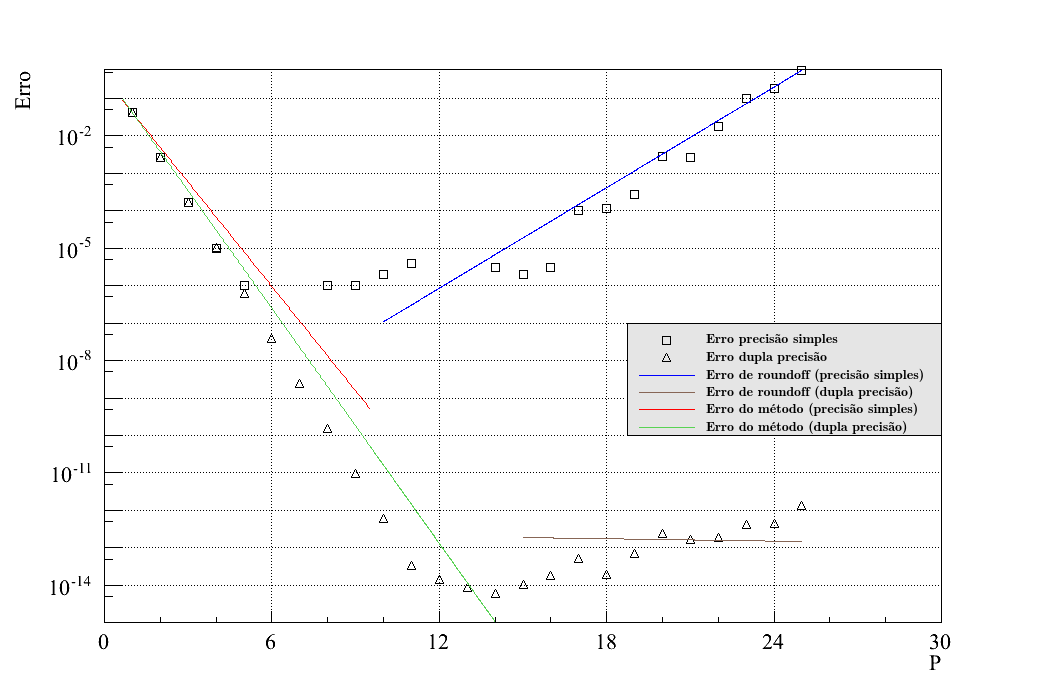
\includegraphics[scale=0.35]{precisao.png}
        \end{center}
        \caption{Gráfico para precisão simples e dupla  .\label{precisao}}
    \end{figure}

    Atrravés do método dos mínimos quadrados é possível ajustar 
    uma função ao conjunto de pontos onde ainda há 
    convergência do valor numérico para o valor literal da integral. Essa função pode ser dada por:
    \begin{equation}
        erro = {\left(\frac{1}{2^p}\right)}^a
    \end{equation}
    onde $a$ é um parametro a ser ajustado.
    Com o ajuste,
    obteve-se os seguintes valores para o parâmetro $a$:
    \begin{eqnarray*}
        \textrm{Para precisão simples} & 3.8\\
        \textrm{Para dupla precisão} & 3.6\\
    \end{eqnarray*}
    O que está proximo da previsão teórica, onde o erro do método é da ordem de $O(h^4)$.
    
    Por outro lado, é possível ajustar outra função, porém, desta vez, ao conjunto de pontos onde o 
    erro passa a aumentar conforme o aumento de partições. Função que pode 
    ser dada por:
    \begin{equation}
        erro = (2^p)^b
    \end{equation}
    onde $b$ é um parametro a ser ajustado.
    Com o ajuste,
    obteve-se os seguintes valores para o parâmetro $b$:
    \begin{eqnarray*}
        \textrm{Para precisão simples} & 0.6\\
        \textrm{Para dupla precisão} & 0.2\\
    \end{eqnarray*}
    O que se assemelha a previsão teórica, onde o erro de roundoff é da ordem de $O(\sqrt{N})$.
    
    \section*{Problema 2}
    O periodo para um pendulo que trabalha dentro de ângulos apreciaveis $(\theta_0 > 10^\circ)$,
    quando se desconsidera a resistência do ar, pode ser dada por:
    \begin{equation}\label{pendulo}
        4\sqrt{\frac{l}{g}}\int^{\pi/2}_0\frac{1}{\sqrt{1 - \sin^2(\theta_0 / 2)\sin^2\theta}}\mathrm{d}\theta
    \end{equation}
    onde $\theta_0$ é o angulo inicial, $l$ o comprimento do pêndulo e $g$ a aceleração da gravidade.
    
    Partindo da equação \eqref{pendulo} é possível implementar um programa que determina o valor do periodo 
    para diferentes valores de $\theta_0$ (20 valores dentro do intervalo $[0, \pi[)$. Programa, este, que utiliza do método
    dos trapézios, o qual divide o intervalo de $[0, \pi/2]$ em 100000 partições, onde, em cada uma delas,
    o ingrando é aproximado por uma reta. O Código do programa segue logo abaixo:
    {\linespread{1.15}
    \lstinputlisting[language=C, label=sqlselect, caption={Implementação 
    para o método do trapézio.}]{pendulo.c}}
    \newpage
    A tabela \ref{tabpendulo} apresenta os valores do periodo para seus respectivos valores de $\theta_0$.
    {\linespread{1}
    \begin{table}[!th]
        \begin{center}
            \begin{tabular}{ c c }
                \toprule[0.11em]
                \n{$\theta_0$ (rad)} & \n{T (s)}\\
                \toprule[0.11em]
                0.000000 & 2.006409 \\
                \midrule
                0.157080 & 2.018821 \\
                \midrule
                0.314159 & 2.057160 \\
                \midrule
                0.471239 & 2.124052 \\
                \midrule
                0.628319 & 2.224411 \\
                \midrule
                0.785398 & 2.368301 \\
                \midrule
                0.942478 & 2.571656 \\
                \midrule
                1.099557 & 2.865801 \\
                \midrule
                1.256637 & 3.320819 \\
                \midrule
                1.413717 & 4.158063 \\
                \midrule
                1.570796 & 65.931862 \\
                \midrule
                1.727876 & 4.158067 \\
                \midrule
                1.884955 & 3.320821 \\
                \midrule
                2.042035 & 2.865802 \\
                \midrule
                2.199115 & 2.571656 \\
                \midrule
                2.356194 & 2.368302 \\
                \midrule
                2.513274 & 2.224411 \\
                \midrule
                2.670354 & 2.124052 \\
                \midrule
                2.827433 & 2.057160 \\
                \midrule
                2.984513 & 2.018821 \\
                \midrule
            \end{tabular}
        \end{center}
        \caption {Valores daequação \eqref{pendulo} para diferentes valores de $\theta_0$.}\label{tabpendulo}
    \end{table}}
    
    Agora, fazendo $\theta_0$ assumir 200 valores diferentes dentro do intervalo $[0, \pi [ $, é possível plotar um gráfico
    do periodo contra $\theta_0$. O qual é apresentado na figura \ref{pendgra}.
    \begin{figure}[!ht]
        \begin{center}
            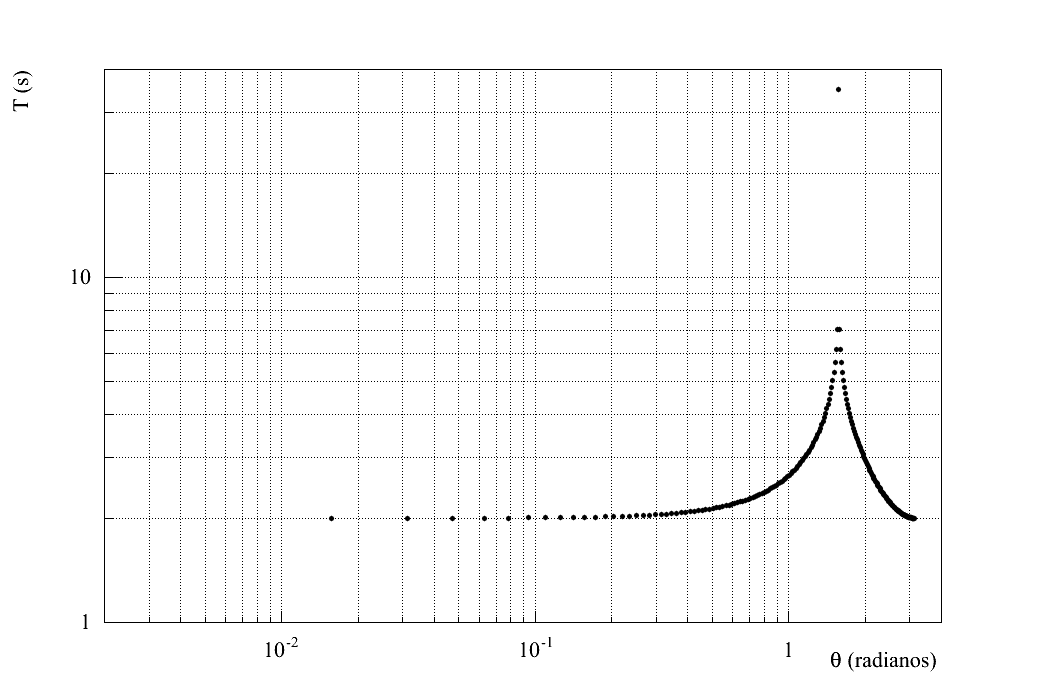
\includegraphics[scale=0.35]{pendulo.png}
        \end{center}
        \caption{Gráfico do periodo em função e de $\theta_0$.}\label{pendgra}
    \end{figure}
    \\[1cm]
    \section*{Problema 3}
    Dado $f(x)$ como:
    \begin{equation}
        f(x) = x^3
    \end{equation}
    é possível determinar a área sobre o gráfico de $f(x)$ no intervalo $0 < x < 1$,
    através do método de Monte-Carlo.
    Para tal, implementou-se um programa que utiliza do ``linear congruential method'' para 
    gerar os números pseudo-aleatórios uniformemente distribuidos. Tomando com semente
    o número 7994808.
    
    O programa se baseia em diferentes números de tentativas, sendo que, em cada tentativa,
    são sorteados 100 pontos ($0 < x < 1$ e $0 < y < 1$). Onde a cada $2^n$ ($1 \le n \le 17 | n \in \mathbb{N}$) tentativas é
    calculado a média das áreas obtidas, o desvio padrão e o desvio padrão da média. O código do pragrama segue logo abaixo.
    {\linespread{1.15}
    \lstinputlisting[language=C, label=sqlselect, caption={Implementação 
    para o método de Monte-Carlo.}]{montecarlo.c}}
    
    A tabela \ref{monte} apresenta os os valores médios da área, o desvio padrão e o desvio padrão da média a cada $2^n$
    tentativas.
    {\linespread{1}
    \begin{table}[!th]
        \begin{center}
            \begin{tabular}{ c c c c }
                \toprule[0.11em]
                \n{$N_t (2^n)$} & \n{$I_m$} & \n{$\sigma$} & \n{$\sigma_m$}\\
                \toprule[0.11em]
                2 & 0.18500 & 0.035 & 0.02041\\
                \midrule
                4 & 0.21250 & 0.038 & 0.01688\\
                \midrule
                8 & 0.22750 & 0.040 & 0.01342\\
                \midrule
                16 & 0.24812 & 0.045 & 0.01085\\
                \midrule
                32 & 0.24563 & 0.044 & 0.00771\\
                \midrule
                64 & 0.24422 & 0.041 & 0.00505\\
                \midrule
                128 & 0.24398 & 0.040 & 0.00348\\
                \midrule
                256 & 0.24418 & 0.039 & 0.00240\\
                \midrule
                512 & 0.24414 & 0.038 & 0.00170\\
                \midrule
                1024 & 0.24406 & 0.038 & 0.00119\\
                \midrule
                2048 & 0.24404 & 0.038 & 0.00084\\
                \midrule
                4096 & 0.24403 & 0.038 & 0.00059\\
                \midrule
                8192 & 0.24404 & 0.038 & 0.00042\\
                \midrule
                16384 & 0.24403 & 0.038 & 0.00030\\
                \midrule
                32768 & 0.24405 & 0.038 & 0.00021\\
                \midrule
                65536 & 0.24405 & 0.038 & 0.00015\\
                \midrule
                131072 & 0.24402 & 0.038 & 0.00011\\
                \midrule
            \end{tabular}
        \end{center}
        \caption {Valores obtidos para o método de Monte-Carlo.}\label{monte}
    \end{table}}
\end{document}